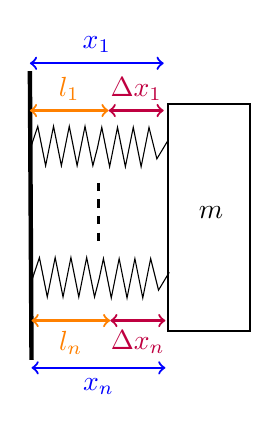
\begin{tikzpicture}
%---------paralelo
\draw [rotate=90] (-1.074,-3.3579) -- (-0.8133,-3.4128) -- (-1.3133,-3.5128) -- (-0.8133,-3.6128) --(-1.3133,-3.7128) -- (-0.8133,-3.8128) -- (-1.3133,-3.9128) -- (-0.8133,-4.0128) -- (-1.2133,-4.1128)-- (-0.9875,-4.249);
\draw [rotate=90] (0.5933,-3.337) -- (0.854,-3.3919) -- (0.354,-3.4919) -- (0.854,-3.5919) --(0.354,-3.6919) -- (0.854,-3.7919) -- (0.354,-3.8919) -- (0.854,-3.9919) -- (0.454,-4.0919)-- (0.6798,-4.2281);
\draw [rotate=90] (-1.1,-2.5) -- (-0.8,-2.6) -- (-1.3,-2.7) -- (-0.8,-2.8) --(-1.3,-2.9) -- (-0.8,-3) -- (-1.3,-3.1) -- (-0.8,-3.2) -- (-1.3,-3.3)-- (-1.074,-3.3579);
\draw [rotate=90] (0.5673,-2.4791) -- (0.8673,-2.5791) -- (0.3673,-2.6791) -- (0.8673,-2.7791) --(0.3673,-2.8791) -- (0.8673,-2.9791) -- (0.3673,-3.0791) -- (0.8673,-3.1791) -- (0.3673,-3.2791)-- (0.5933,-3.337);
\draw [ultra thick](2.4791,1.5673) -- (2.5,-2.1);
\draw [thick] (4.2369,1.1484) rectangle (5.2791,-1.7327);
\node at (4.7791,-0.2327) {$m$};
\draw [thick, <->, orange] (2.4791,1.0673) -- (3.4791,1.0673)node [midway, above]{$l_1$};
\draw [thick, <->, orange] (2.5,-1.6) -- (3.5,-1.6)node [midway, below]{$l_n$};
\draw [thick, <->, purple] (3.4791,1.0673) -- (4.1791,1.0673)node [midway, above]{$\Delta x_1$};
\draw [thick, <->, purple] (3.5,-1.6) -- (4.2,-1.6)node [midway, below]{$\Delta x_n$};
\draw [thick, <->, blue](2.4791,1.6673) -- (4.1791,1.6673)node [midway, above]{$x_1$};
\draw [thick, <->, blue](2.5,-2.2) -- (4.2,-2.2)node [midway, below]{$x_n$};
\draw [ thick, dashed] (3.35,0.15) -- (3.35,-0.6);

\end{tikzpicture}